

\definecolor{tiffanyblue}{RGB}{129,216,208}
\definecolor{bangdiblue}{RGB}{0,149,182}
\definecolor{kleinblue}{RGB}{0,47,167}
\definecolor{kabuliblue}{RGB}{26,85,153}
\definecolor{purple}{RGB}{138,43,226}
\usepgfplotslibrary{groupplots}
\usepgfplotslibrary{fillbetween} 
\begin{figure*}[t!]
  \centering
  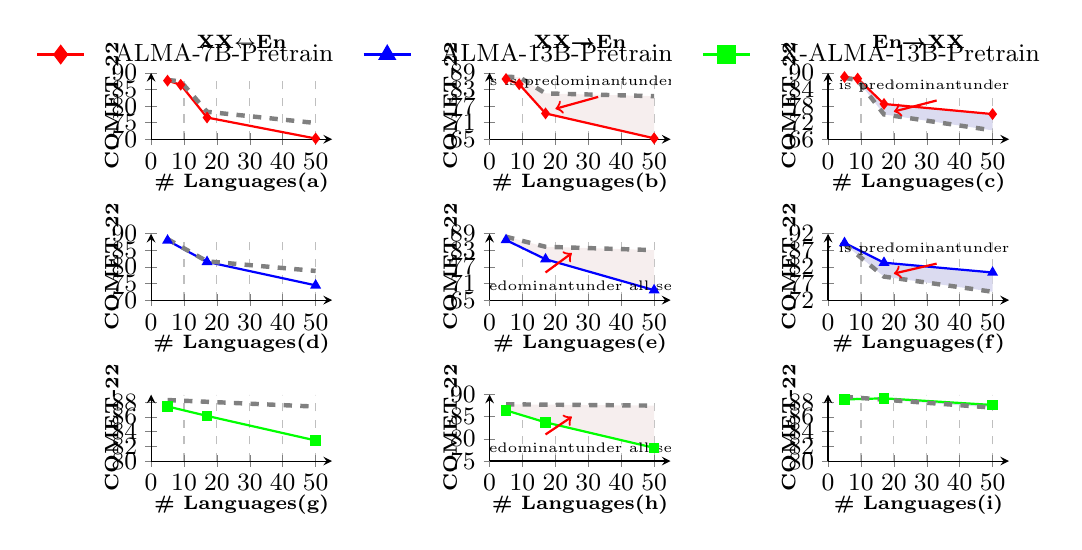
\begin{tikzpicture}
    \pgfplotsset{set layers}
    \scriptsize{
    % 全局图例单独绘制
    \begin{axis}[
    at={(2,1.4)},
    width=0.5\textwidth,
      height=0.2\textwidth,
      hide axis,
      xmin=0, xmax=0.5, ymin=0, ymax=0.5,
      legend style={
        draw=none,
        fill=none,
        font=\small,
        column sep=0.3cm,
        at={(1.1,1.6)},
        anchor=north
      },
      legend columns=3
    ]
      \addlegendimage{red, mark=diamond*, mark size=3.0pt, thick, mark options={solid, fill=red}}
      \addlegendentry{ALMA-7B-Pretrain}
      \addlegendimage{blue, mark=triangle*, mark size=3.0pt, thick, mark options={solid, fill=blue}}
      \addlegendentry{ALMA-13B-Pretrain}
      \addlegendimage{green, mark=square*, mark size=3.0pt, thick, mark options={solid, fill=green}}
      \addlegendentry{X-ALMA-13B-Pretrain}
    \end{axis}
    }
    \scriptsize{
    \begin{groupplot}[
      group style={group size=3 by 3, horizontal sep=2cm, vertical sep=1.2cm},
      xmajorgrids,
      grid style={dashed, gray!50},
      width=0.32\textwidth,
      height=0.2\textwidth,
      xlabel={\# Languages},
      ylabel={COMET-22},
      xlabel style={font=\bfseries, yshift=0.5em},
      ylabel style={font=\bfseries, yshift=-1.0em},
      yticklabel style={font=\small},
      xticklabel style={font=\small},
      title style={font=\bfseries},
      xmin=0, xmax=55, 
      xtick={0, 10, 20, 30, 40, 50},
        axis x line=bottom,
        axis y line=left,
        % axis y line*=left, % 左Y轴
    ]
    % 第一行:Model 1
    \nextgroupplot[title={XX$\leftrightarrow$En}, xlabel={\makecell{\# Languages \\ (a) } },ymin=70, ymax=90, ytick={70, 75, 80, 85,90}]
    \addplot[red, mark=diamond*, mark size=1.5pt, thick, mark options={solid, fill=red}] 
      coordinates {(5, 87.64) (9, 86.41) (17, 76.54) (50, 70.22)};
    \addplot[ultra thick, dashed, gray] 
      coordinates {(5, 87.86) (9, 87.42) (17, 78.27) (50, 74.89)};
      
    \nextgroupplot[title={XX→En}, xlabel={\makecell{\# Languages \\ (b) } }, ymin=65, ymax=89, ytick={65, 71, 77, 83, 89}]
    \addplot[name path=mt_b,red, mark=diamond*, mark size=1.5pt, thick, mark options={solid, fill=red}] 
      coordinates {(5, 86.76) (9, 84.89) (17, 74.33) (50, 65.35)};
    \addplot[name path=separate_b,ultra thick, dashed, gray] 
      coordinates {(5, 87.53) (9, 87.48) (17, 81.57) (50, 80.57)};
    
    \addplot [
        fill=red!30!gray!10
    ] fill between [
        of=mt_b and separate_b,
    ];

    \draw[->, thick, color=red] (axis cs:33,80.3) node[above]{\tiny \textcolor{black}{\makecell{Conflicts is predominant\\ under all settings}}} -- (axis cs:20,76);


    
    \nextgroupplot[
        title={En→XX}, 
        xlabel={\makecell{\# Languages \\ (c) } }, 
        % 左 Y 轴(COMET-22)
        ylabel={COMET-22}, 
        ymin=66, ymax=90, 
        ytick={66, 72, 78, 84, 90},
    ]
    \addplot[name path=mt_c, red, mark=diamond*, mark size=1.5pt, thick, mark options={solid, fill=red}] 
      coordinates {(5, 88.52) (9, 87.92) (17, 78.75) (50, 75.09)};
    \addplot[name path=separate_c,ultra thick, dashed, gray] 
      coordinates {(5, 88.19) (9, 87.35) (17, 74.97) (50, 69.21)};

    \addplot [
        fill=blue!40!gray!20
    ] fill between [
        of=mt_c and separate_c,
    ];

    \draw[->, thick, color=red] (axis cs:33,80) node[above]{\tiny \textcolor{black}{\makecell{Synergy is predominant\\ under all settings}}} -- (axis cs:20,76)
         ;

   
    
    
    % 第二行:Model 2
    \nextgroupplot[xlabel={\makecell{\# Languages \\ (d) } }, ymin=70, ymax=90, ytick={70, 75, 80, 85, 90}]
    \addplot[blue, mark=triangle*, mark size=1.5pt, thick, mark options={solid, fill=blue}] 
      coordinates {(5, 87.97) (17, 81.53) (50, 74.46)};
    
    % \addplot[ultra thick, dashed, gray] 
    %   coordinates {(5, 88.40) (9, 88.57) (17, 81.692) (50, 78.80)};

    \addplot[ultra thick, dashed, gray] 
      coordinates {(5, 88.40) (17, 81.692) (50, 78.80)};
    
    \nextgroupplot[xlabel={\makecell{\# Languages \\ (e) } }, ymin=65, ymax=89, ytick={65, 71, 77, 83, 89}]
    \addplot[name path=mt_e, blue, mark=triangle*, mark size=1.5pt, thick, mark options={solid, fill=blue}] 
      coordinates {(5, 86.72) (17, 79.79) (50, 68.60)};

    % \addplot[ultra thick, dashed, gray] 
    %   coordinates {(5, 87.92) (9, 88.068) (17, 84.289) (50, 83.079)};
      \addplot[name path=separate_e, ultra thick, dashed, gray] 
      coordinates {(5, 87.92) (17, 84.289) (50, 83.079)};

     \addplot [
        fill=red!30!gray!10
    ] fill between [
        of=mt_e and separate_e,
    ];

    \draw[->, thick, color=red] (axis cs:17,75) node[below]{\tiny \textcolor{black}{\makecell{Conflicts is predominant\\ under all settings}}} -- (axis cs:25,82)
         ;
     
    \nextgroupplot[xlabel={\makecell{\# Languages \\ (f) } },ymin=72, ymax=92, ytick={72, 77, 82, 87, 92}]
    \addplot[name path=mt_f,blue, mark=triangle*, mark size=1.5pt, thick, mark options={solid, fill=blue}] 
      coordinates {(5, 89.23) (17, 83.28) (50, 80.33)};

     % \addplot[ultra thick, dashed, gray] 
     %  coordinates {(5, 88.882) (9, 89.071) (17, 79.095) (50, 74.52)};

      \addplot[name path=separate_f,ultra thick, dashed, gray] 
      coordinates {(5, 88.882)  (17, 79.095) (50, 74.52)};

      \addplot [
        fill=blue!40!gray!20
    ] fill between [
        of=mt_f and separate_f,
    ];

    \draw[->, thick, color=red] (axis cs:33,83) node[above]{\tiny \textcolor{black}{\makecell{Synergy is predominant\\ under all settings}}} -- (axis cs:20,80)
         ;

    % 第三行:Model 3
    \nextgroupplot[xlabel={\makecell{\# Languages \\ (g) } }, ymin=80, ymax=89, ytick={80, 82, 84, 86, 88}]
    \addplot[green, mark=square*, mark size=1.5pt, thick, mark options={solid, fill=green}] 
      coordinates {(5, 87.40) (17, 86.12) (50, 82.79)};
    \addplot[ultra thick, dashed, gray]  coordinates {(5, 88.27) (50, 87.38)};

    
    \nextgroupplot[xlabel={\makecell{\# Languages \\ (h) } }, ymin=75, ymax=90, ytick={75, 80, 85, 90}]
    \addplot[name path=mt_h,green, mark=square*, mark size=1.5pt, thick, mark options={solid, fill=green}] 
      coordinates {(5, 86.45) (17, 83.74) (50, 77.98)};
    \addplot[name path=separate_h, ultra thick, dashed, gray] 
      coordinates {(5, 87.82) (50, 87.52)};
    % \node at (0.5,-10.25) {(c) XX-En};

    \addplot [
        fill=red!30!gray!10
    ] fill between [
        of=mt_h and separate_h,
    ];

    \draw[->, thick, color=red] (axis cs:17,81) node[below]{\tiny \textcolor{black}{\makecell{Conflicts is predominant\\ under all settings}}} -- (axis cs:25,85)
         ;
    
    \nextgroupplot[xlabel={\makecell{\# Languages \\ (i) } },ymin=80, ymax=89, ytick={80,82, 84, 86, 88}]
    \addplot[name path=mt_i,green, mark=square*, mark size=1.5pt, thick, mark options={solid, fill=green}] 
      coordinates {(5, 88.35) (17, 88.50) (50, 87.60)};
      \addplot[name path=separate_i, ultra thick, dashed, gray]  coordinates {(5, 88.71) (50, 87.24)};

    \addplot [
        fill=blue!40!gray!20
    ] fill between [
        of=mt_i and separate_i,
    ];

    
    \end{groupplot}
    }
  \end{tikzpicture}
  \vskip -0.1in
  \caption{Performance of different models trained on varying numbers of languages. The dotted line represents the performance of separately trained models, serving as a reference point where no language conflicts or synergies occur. Two key findings emerge: (1) Asymmetry in Linguistic Conflicts and Synergy (Figure a–i), highlighting the uneven impact of multilingual training across language pairs; and (2) The Bottleneck of Multilinguality in Post-Training (Figure g–i): While multilingual pre-training provides a solid foundation for handling multiple languages, the multilingual training phase can lead to the CoM.}
  \label{fig:Asymmetric_Conflict_and_Synergy}
\end{figure*}

